\chapter{BENZER MİMARİLER VE ÖNCEKİ ÇALIŞMALAR}
Gereksinimlerde belirtilen fonksiyonlar ışığında hesaplamalar için kullanılacak modüller belli IPCore donanımları ve basit hesaplama modüllerinden oluşur. Paralel işlemeye özel donanımlarda yürütme zamanının en büyük bileşeni verilerin okunması ve yazılmasından oluşan bellek işlemleri olduğu için mimari seviyesinde donanım özelliklerini belirleyici unsur, veri yolu tasarımıdır.\par

Veri yolu mimarisi, bellek, yazmaç öbekleri ve hesaplama birimleri arasındaki bağlantı ile bu yapıların mimari hiyerarşisinden oluşur. Literatürde öne çıkan veri yolu mimarileri üç sınıfta değerlendirilebilir: Homojen az çekirdekli işlemciler, homojen çok çekirdekli işlemciler ve heterojen yapıdaki işlemciler. \par

\subsection{Homojen az çekirdekli işlemciler}
Homojen az çekirdekli mimariler birbirinin aynı olan az sayıda çekirdeklerin 2. veya daha üst seviyede önbellekler üzerinden veri paylaşımı sağladığı işlemcilerdir. Bu mimaride her işlemci çekirdeğin kendisine ait bir önbelleği vardır. Bunlar bir interconnect yardımıyla bütünleşik bir paylaşımlı önbelleğe bağlanırlar. Bu yapı Intel'in Nehalem işlemcilerindeki yapı ile uyumluluk gösterir \cite{molka2009memory} \cite{hackenberg2009comparing}. Nehalem mimarisinde özel önbellek 2 seviyeye ayrılmıştır ve paylaşımlı önbellek 3. seviyeyi oluşturmaktadır. Daha sonra çekirdek Şekil \ref{image:nehalem}'deki gibi bir bellek denetleyicisi ile sistemin ana belleğine bağlanmaktadır.\par

\begin{figure}[h] \label{image:nehalem} 
\centering 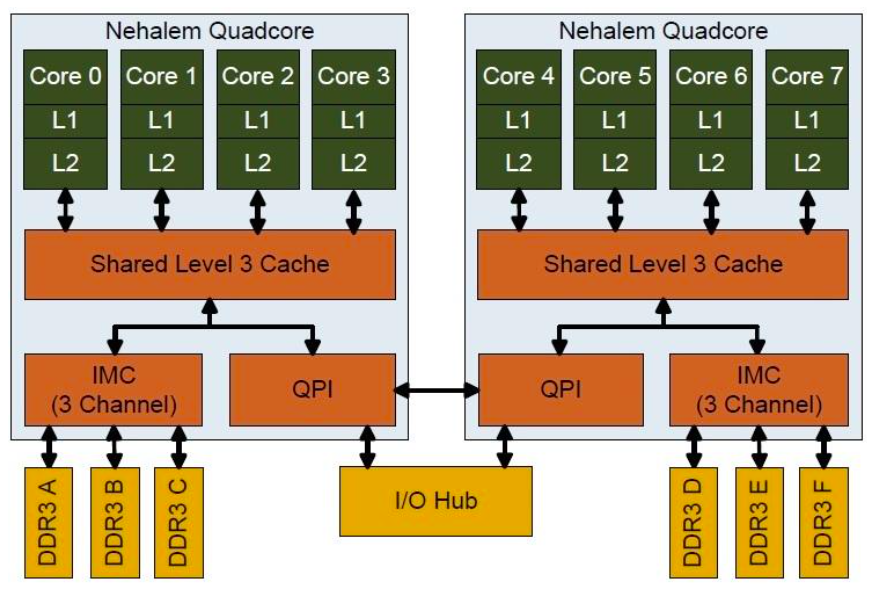
\includegraphics[width=\textwidth]{gorsel/nehalem.jpg} \caption{Nehalem}  
\end{figure}